\documentclass[10pt,]{book}
\usepackage{amssymb,amsmath}
\usepackage{ifxetex,ifluatex}
\usepackage{microtype}
\usepackage{fixltx2e} % provides \textsubscript
\linespread{1.3}
\ifxetex
  \usepackage{fontspec,xltxtra,xunicode}
  \defaultfontfeatures{Mapping=tex-text,Scale=MatchLowercase}
  \newcommand{\euro}{€}
\else
  \ifluatex
    \usepackage{fontspec}
    \defaultfontfeatures{Mapping=tex-text,Scale=MatchLowercase}
    \newcommand{\euro}{€}
  \else
    \usepackage[utf8]{inputenc}
  \fi
\fi
\usepackage{biblatex}
\bibliography{Thesis}
\usepackage{listings}
\lstset{basicstyle=\footnotesize\ttfamily}
\usepackage{fancyvrb}
% Redefine labelwidth for lists; otherwise, the enumerate package will cause
% markers to extend beyond the left margin.
\makeatletter\AtBeginDocument{%
  \renewcommand{\@listi}
    {\setlength{\labelwidth}{4em}}
}\makeatother
\usepackage{enumerate}
\usepackage{ctable}
\usepackage{float} % provides the H option for float placement
\ifxetex
  \usepackage[setpagesize=false, % page size defined by xetex
              unicode=false, % unicode breaks when used with xetex
              xetex,
              bookmarks=true,
              pdfauthor={},
              pdftitle={},
              colorlinks=true,
              urlcolor=blue,
              linkcolor=blue]{hyperref}
\else
  \usepackage[unicode=true,
              bookmarks=true,
              pdfauthor={},
              pdftitle={},
              colorlinks=true,
              urlcolor=blue,
              linkcolor=blue]{hyperref}
\fi
\hypersetup{breaklinks=true, pdfborder={0 0 0}}
\setlength{\parindent}{0pt}
\setlength{\parskip}{6pt plus 2pt minus 1pt}
\setlength{\emergencystretch}{3em}  % prevent overfull lines
\setcounter{secnumdepth}{0}
\VerbatimFootnotes % allows verbatim text in footnotes

\title{Platform Independent Programs}
\author{Joseph
                Hallett\thanks{With thanks to Dr. Daniel Page for supervising the project and to Will Williams and Jake Longo for listening to me rant about PIPs and byte-code all year.}}
\date{\today}

\widowpenalty=300
\clubpenalty=300
\usepackage{epigraph}
\begin{document}
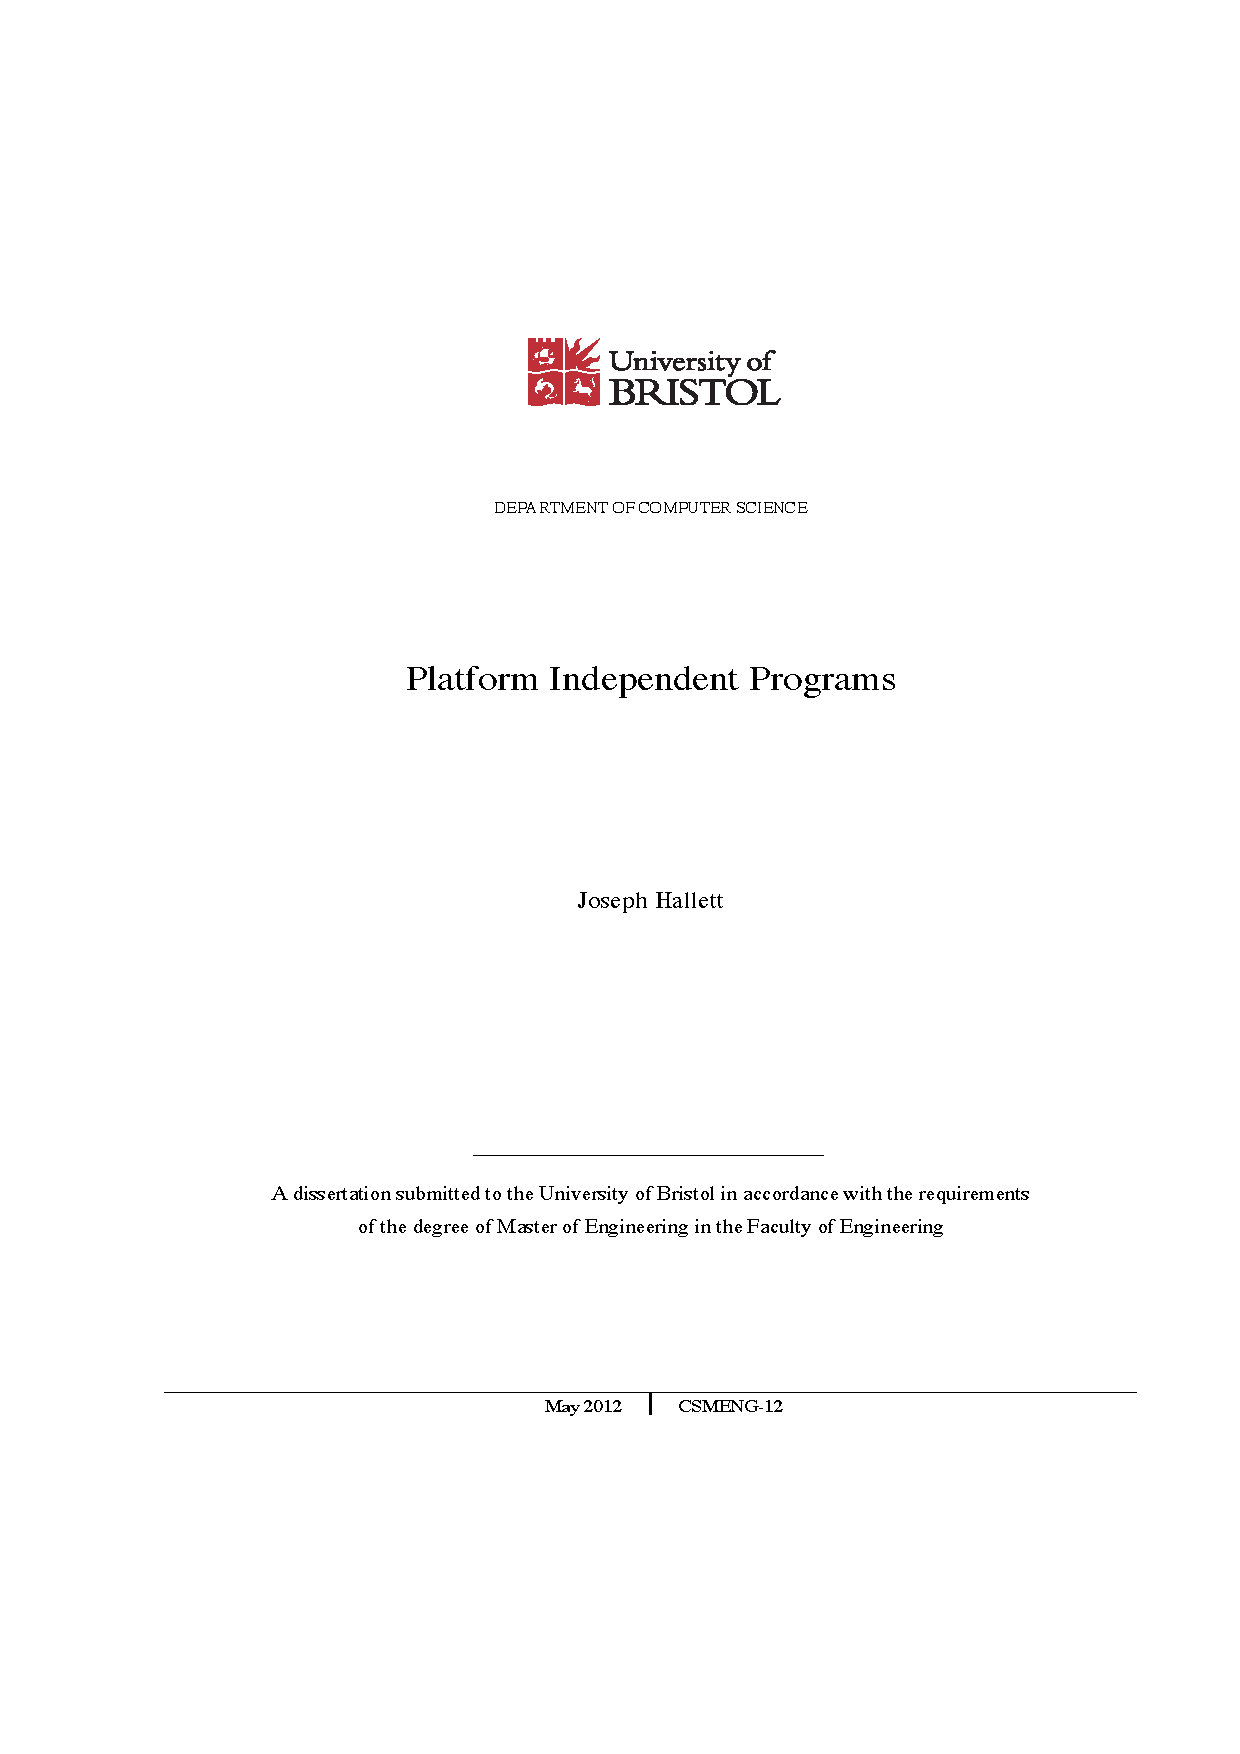
\includegraphics[width=\linewidth]{Cover.pdf}

\includegraphics[width=\linewidth]{Declaration.pdf}


\maketitle

\epigraph{\textsf{``{.}{.}{.}a large, flat space to spread out the architecture reference manuals, and an ample supply of caffeine. Do not underrate the second part."}}{\textsf{Drew Dean}}

\tableofcontents
\listoftables
\lstlistoflistings
\chapter{Executive Summary}

\emph{Platform Independent Programs} (PIPs) are a new type of program
whose byte-code can be run on multiple architectures without
modification. By exploiting overlaps between architectures of their
compiled instruction formats it is possible to create small sequences of
code called, PIP headers, that jump to different places depending on
which architecture runs them. By chaining the PIP headers with jumps to
platform specific code you can construct whole programs that run on
multiple architectures.

I created a database of semantic NOP (no-operation) instructions for the
ARM, MIPS, X86 and XS1 architectures and used it to find PIP headers for
the ARM, MIPS and X86 platforms and to show the technique is also
possible on XS1. I improved upon the existing attempts to find four byte
PIPs for the MIPS platform, and found approximately the same number for
every other architecture. I looked at the steganographic properties of
PIPs and the occurrences of PIP headers in non PIP programs. I
determined that using repeated PIP headers would lead to a PIP that was
easily distinguished from a non PIP by statistical methods. I suggested
other methods to create PIPs that could not be detected by a signature
based scheme by using metamorphism, encryption, and microcode updates. I
created an example shellcode using a PIP header that highlighted the
need for some form of static analysis to be introduced to the PIP header
generation routine to fully utilize PIPs.

\chapter{Introduction}

\section{Constructing PIPs}

In 2010 a team of researchers developed a generalised method for
creating Platform Independent Programs (PIPs)\autocite{Cha:2010uh}. A
PIP is a special sort of program which can be run on multiple different
computer architectures without modification. Unlike shell scripts or
programs written for a portable interpreter; a PIP does not require
another program to run or compile it; rather it runs as a native program
on multiple architectures with potentially different behaviours on each.

A more formal definition of a PIP is a string of byte-code $b$ such that
for different machines $m_1$ and $m_2$, $b$ is a valid program if:

\[m_1(b) \not = \bot \wedge m_2(b) \not =\bot.\]

To construct a PIP one must analyse the instruction sets of each
architecture and find instructions which compile to identical patterns
of byte-code. The approach taken by the authors in \autocite{Cha:2010uh}
was to find small PIPs with a very specific form: do nothing then jump.
By ensuring each architecture jumped to a different point and that each
architecture did not accidentally run into a region another architecture
jumped into; they could construct PIPs for any arbitrary program by
splitting them up into blocks of instructions specific to each
architecture and connecting them with the small PIPs.

Consider the following example (taken from \autocite{Cha:2010uh}). The
disassembly for the X86 architecture is shown above, and for the MIPS
platform below.

\[\underbrace{\overbrace{90}^{\text{NOP}} \overbrace{eb20}^{\text{JMP}}
2a }_{\text{NOP}} \underbrace{90eb203a}_{\text{NOP}}
\underbrace{24770104}_{\text{B}}\]

The string is valid on both platforms and has similar behaviour on both
despite jumping to different locations. In fact this is a valid PIP for
the X86, MIPS and ARM architectures. If we disassemble the pattern with
the Radare2 reverse engineering framework\autocite{radarenopcodeorg:vw}
we can see that it disassembles to:

\ctable[caption = Disassembly of an example PIP header from
\autocite{Cha:2010uh}, pos = H, center, botcap]{ll}
{% notes
}
{% rows
\FL
Architecture & Disassembly
\ML
X86 & \lstinline!nop; jmp 0x100000023; sub dl, [eax+0x243a20eb]; ja 0x10000000c; ???!
\\\noalign{\medskip}
ARM & \lstinline!bcs 0x10083ae48; bcc 0x10083ae4c; streq r7, [r1], #-1828!
\\\noalign{\medskip}
MIPS & \lstinline!slti zero,s1,-5232; xori zero,s1,0xeb90; b 0x10001dc9c!
\LL
}

For the X86 architecture it is a NOP instruction then a jump
instruction. The rest wont be executed (though some of it is valid X86
code) as the unconditional jump will have moved the program counter
along. For the ARM architecture it starts with two conditional jumps.
The first tests if the processor's carry flag is set, and the next
checks if the carry flag is not set. One of these two instructions will
be executed so one of the two jumps will be taken. For MIPS architecture
the first two instructions write the result of the operation back to
register zero. On the MIPS architecture any writes to register zero are
discarded and the \lstinline!slti! and \lstinline!xori! can not cause
any errors to occur. This means the first two instructions are
equivalent to a \lstinline!NOP! instruction. The third instruction is a
MIPS branch instruction, so the sequence for a MIPS computer is
equivalent to do nothing and jump.

Since for each of the X86, ARM, and MIPS architectures the byte-code is
equivalent to do nothing and jump; the instruction is a valid PIP.

They go on to give a generalised algorithm for constructing these PIPs,
and say that they have a working implementation of it for creating PIPs
for the X86, ARM, and MIPS platforms, as well as the Windows, Mac, and
Linux operating systems.

\section{Aim Of The Project}

For this thesis I have implemented a section of the PIP finding
algorithm: the section for finding the \emph{gadget headers}; the PIPs
that link the specific code sections together. To generate the PIPs a
list of \emph{semantic NOPs}\footnote{A semantic NOP is an instruction
  which has no effect, but which might not necessarily be the \emph{NOP}
  assembly instruction. For example the ARM instruction:
  \lstinline!MOV r4, r4! Causes the contents of register four to be
  moved into register four and as such is equivalent to an actual
  \lstinline!NOP! instruction. Equally the sequence of instructions:
  \lstinline!PUSH r3! \lstinline!POP r3! is equivalent to two
  \lstinline!NOP! instructions when taken as a whole and so is a
  \emph{multi-instruction semantic NOP}.} and potential branch
instructions has been found for each the ARM, X86 and MIPS
architectures. These have been compiled into a list of PIP headers for
each of the architectures.

Unfortunately there does not seem to be a public database of the
semantic NOP instructions required for PIP generation. Semantic NOPs
have been used in areas other than creating PIPs, for example malware
classification\autocite{Bilar:2007uu}\autocite{Preda:2007ky}, but there
still appears to be no exhaustive list documenting them. I have created
one and made it publicly available.

To extend the work of the original paper\autocite{Cha:2010uh} I have
also looked at how often PIPs headers turn up \emph{in the wild} in
regular non-PIP code. This is important as PIPs have some steganographic
properties. If PIP can be distinguished from non-PIP then this may
affect how suitable PIPs are for use in a steganographic system.

\section{Applications Of PIPs}

PIPs can be used for a variety of applications. One potential
application suggested by Brumley et. al.\autocite{Cha:2010uh} is for
sneaking programs past dynamic execution checkers. Suppose two prisoners
\emph{Alice} \& \emph{Bob}, wish to send a malicious program between
themselves. To send the message they have to send it through a
\emph{Warden} who checks first that there communications do not contain
anything malicious and only delivers the message if its believed to be
harmless.

Steganography is the science of \d{h}iding
information\autocite{Gordon:vw}. It has been used in parall\d{e}\d{l}
with cryptography to hide messages in seeming\d{l}y inn\d{o}cuous
docu\d{m}ents\autocite{Saamuson:wt}, to circumvent b\d{a}ns on
cryptog\d{r}aphy\autocite{Owens:2002uq}, and \d{t}o \d{i}mplement
watermarking\autocite{Wayner:2009vw}. To sneak the program Alice and Bob
use a form of \emph{keyed-steganography}\footnote{which the
  authors\autocite{Cha:2010uh} call \emph{execution-based
  steganography}.}. The program which they wish to communicate becomes
their \emph{steg-text}, and they construct a \emph{cover-text} by
writing some other program which does not contain anything malicious.
They pre-arrange a shared secret which is the platform that their
programs should really be run on: this forms the key. With the
cover-text and steg-text created they create their message by generating
them into a PIP where on one platform (X86 say) it appears to run the
innocuous program and on the secret key platform (ARM for the sake of
argument) it runs the program they really wish to communicate. Alice
hands the warden the program and tells him that it is for the innocuous
architecture\footnote{if they were using ELF they would not even need to
  do that---it is part of the header in the file\autocite{mancx:th}.}.
The warden runs the program and sees it is not something he would want
to restrict and delivers it. In fact unless he is aware that it has been
in constructed in this way he may not even check any other architectures
as for most platforms it will appear to be garbage \d{j}ust like a\d{n}y
norm\d{a}l executable.

A more real world example of this is to co\d{n}si\d{d}er the
relationship between computer\d{s} (usually us\d{i}ng an X86 processor)
and \d{m}odern smart ph\d{o}nes (which ofte\d{n} use ARM processors)
running \emph{apps}. The computer often stores backups of the
applications used on the smartphone. Apple's iTunes program, for
example, stores all the mobile applications associated with a user in it
is library folder as zip-compressed archives. Suppose an attacker were
to construct a program which was a legitimate application on the ARM
platform but when run on X86 behaved as a form of malware. The computer
might have some form of anti-malware software, but unless it knows to
scan the mobile applications as potential X86 viruses rather than the
ARM ones they identify themselves as (and which are not ARM malware)
then the anti-malware program might miss the dangerous code.

Another application is \emph{exfiltration protection}. Exfiltration is a
military term meaning the removal of a resource from enemy control. In
the context of PIPs this probably involves taking programs from
protected PCs; similar to DRM. The idea is that to protect its software
from theft a secret agency could make a modification to an existing
platform (the JVM or another virtual machine would be a good choice
here) and compile their program for this modified platform. They then
create another program for the unmodified platform which does something
else; maybe it phones home, maybe it destroys itself from the computer
it is running on. They create a PIP out of these two programs and now if
the program is stolen and the exfiltrator is not aware of the PIP nature
(or exactly what modifications were made to the architecture) they
cannot execute the program they removed.

Microcode offers another interesting way to use PIPs. Suppose an
attacker manages to compromise a system in such a way that they can
alter the microcode of the processor, such as the recent HP printer
attack amongst others\autocite{Cui:vx}\autocite{Scythale:tk}. Now
suppose that as well as the microcode update they also modify an
existing program, Brumley et. al. suggest \lstinline!ls!, so that on the
compromised system it gives a backdoor or acts maliciously, but on
another (say one which is trying to forensically work out what is wrong
with the printer) it acts normally. Brumley et. al. point
out\autocite{Cha:2010uh} that if this was done by Intel and the PIP was
a preexisting and digitally signed application: it is a particularly
scary prospect. Merely signing the program would be insufficient to
protect a user it would not check if the machine it was executing on had
been modified.

PIPs could also be used to create platform independent shell code to
take advantage of buffer overflows on software ported between different
architectures and operating systems. As well as developing PIPs to
create architecture independent programs, Brumley et.
al.\autocite{Cha:2010uh} extended the basic technique to create
operating system programs. For operating system independent programs
they exploited overlaps in calling conventions and interrupts to develop
PIPs which could be valid programs on multiple systems. Brumley et. al.
give an example of a remote bind-shell shell code for multiple
architectures at the end of their paper \autocite{Cha:2010uh}.

Another application for PIPs is to create actual platform independent
programs. The idea here is to compile a program for multiple
architectures and create a PIP out of them. You would get a program that
behaved the same but ran on multiple architectures. This could be
useful, for example, if you have a network of computers (some Linux X86
based, some ARM based) and you want to run a server hosting all the
programs to share between them you do not have to maintain multiple
versions.

\section{Other Approaches To Program Obfuscation}

The problem is that although PIPs could be used to write architecture
independent programs, there are more elegant solutions available than
relying on the intersection of instruction sets between architectures.
There are several preexisting systems for doing this such as Apple's
\emph{Universal Binary} or the \emph{FatELF}\autocite{Icculus:vl}
format. Another problem is that for some operating systems this just
would not work: Linux normally uses the ELF format\autocite{mancx:th}
which has a flag in the header which specifies exactly what architecture
the binary was compiled for. If it does not match the architecture of
the machine it is being run on, then the loader refuses to run
it\footnote{Of course there is nothing to stop you flipping the flag to
  some other value with \lstinline!elfedit! utility from the GNU
  Binutils.}.

Collberg et. al. \autocite{Collberg:1997vt} describe different methods
for hiding the structure of a program. They give many different
transforms but three are of particular interest: adding dead code,
adding redundant transforms, and outlining\footnote{Outlining is the
  opposite of inlining. For inlining we take a function call and replace
  it with the functions code inserted into the main program verbatim.
  For outlining we take a block of code inside a function and make a
  function call out of it. You might do inlining to skim a couple of
  jump instructions from our program at the expense of a longer program;
  but outlining (especially of sections only run once) just adds to the
  spaghetti nature of the code.} sections of code.

These three are of interest because they describe what a PIP is doing,
namely adding redundant NOPs and transforms which do not alter the state
of the program before jumping to the actual code.

Whilst adding the \lstinline!NOP! instructions is not a particularly
\emph{resilient}\footnote{Resilience is a measure of how easy it is to
  deobfuscate a transform. It is usually measured in terms of the time
  and space the deobfuscator has to run.} transformation (a program
could replace or remove them) they are potent\footnote{Potency measures
  how confusing for a human the transform is. For example self-modifying
  code is a very potent transform, but renaming the jump targets is not.}
especially if they are combined with multi-instruction semantic NOPs
where the state of the program does change only to be reversed later.
The jumps added by the PIPs act to outline blocks of code. If you are
using just one PIP at the start of the program then the amount of
obfuscation is minimal; but in a situation where you are outlining every
single instruction with a PIP like structure and possibly embedding
different behaviour if it is run on a different architecture (such as
Java or Thumb mode on an ARM chip) this has the potential to be
massively obfuscating.

Interestingly papers, such as
\autocite{Christodorescu:2005vh}\autocite{Christodorescu:2005vf}, even
describe obfuscation techniques where they deobfuscate the addition of
semantic NOPs using a novel (and patented
\autocite{Christodorescu:2009wo}) tool called \emph{Hammock}. Hammock
appears to be interesting because rather than using a catalogue of
pre-known semantic NOPs it finds them by analysing whether sequences of
code have any net effect on the state of the machine. They find it to be
a very slow transform to deobfuscate (implying adding NOPs is a potent
obfuscation technique) but the removal is quick once they have been
found.

Semantic NOPs are another interesting aspect of the PIP problem.
Semantic NOPs are important for PIPs as they give you multiple ways of
doing nothing---so there is a greater chance of finding an overlap
between different architectures but they turn up in other places too.
Many people
\autocite{Christodorescu:2005vh}\autocite{Owens:2011um}\autocite{Bruschi:2007dn}
have suggested using semantic NOPs as an obfuscating technique. Wartell
et. al.\autocite{Wartell:2011ji} suggest using them as part of a
heuristic for differentiating between code and data for disassembled
programs. The GNU Assembler has a short list of efficient, low power
semantic NOP\footnote{A comment above the
  function\autocite{Anonymous:td} notes that most of the instructions
  used as part of the semantic NOP sequences by the assembler are not in
  fact assemblable with the assembler.} instructions it uses to pad
instruction sequences to cache-lines\autocite{Anonymous:td}.

\section{What Is The Challenge?}

The original PIP paper\autocite{Cha:2010uh} contains an anecdote where
the effort required to create platform independent programs is described
as requiring:

\begin{quote}
``a large, flat space to spread out the architecture reference manuals,
and an ample supply of caffeine. Do not underrate the second part.''

\end{quote}
Brumley et al go on to note that:

\begin{quote}
``even the most caffeinated approaches have only been met with limited
success;''

\end{quote}
For this thesis I am not trying to fully generate platform independent
programs; rather I am trying to find the headers that enable them. To do
this I need two things: a list of semantic NOP And jump instructions for
each architecture I wish to find PIPs for; and a method for combining
them to form the headers.

Finding the semantic NOPs and jump instructions in theory is quite easy.
You can go through the architecture manual making notes of the all the
instructions which you are interested in (checking that they do not
alter the state of the processor in any surprising way) before
assembling them to get the byte-code. For some architectures it
\emph{is} easy---the instruction sets are small and everything in the
instruction set is accessible through a standard assembler.

The MIPS architecture\autocite{MIPSTechnologiesInc:2011ta} is a good
example of a platform where finding semantic NOPs is easy. A short RISC
instruction set, a limited number of status-altering instructions and a
register that discards any value written to it make it and ideal
platform for writing semantic NOPs. Several million single instruction
semantic NOPs can be found with minimal effort. The Intel X86
architecture\autocite{IntelCorporation:1997ta} is completely different
however. There are a large number of instructions here including
multiple forms of the same instructions which the assembler is free to
pick between. All arithmetic instructions alter status flags. Worse
still there are some assembly instructions that can not be assembled by
the GNU tool chain\autocite{Anonymous:td}. It is considerably harder to
find semantic NOPs for the X86 architecture.

Once I know the form of the instructions I want to assemble I need to
compile and disassemble them to get the byte-code, and store them in a
database. Once I have them in an indexable format I will need to search
for the patterns that overlap and find all the PIP headers. There are
significant problems associated with finding these PIP headers. For
platforms like ARM\autocite{Seal:2000vd} and
MIPS\autocite{MIPSTechnologiesInc:2011ta} instructions are all compiled
to be of fixed length (four bytes). In this case I could find short PIPs
by comparing the lists of NOP instructions for one architecture and jump
instructions for the other. You could extend them to arbitrary lengths
by finding the NOPs which do nothing on both architectures and padding
to the length required.

In practice however this approach does not work. Variable length
instruction sets, such as X86\footnote{For example the instruction
  \lstinline!NOP! compiles to \lstinline![0x90]!, but the
  \lstinline!movsldup xmm0,xmm1! instruction becomes
  \lstinline![0xF3, 0x0F, 0x12, 0xC1]!.}, mean you need to combine
instructions together to get them to the length you require. If there
were only a few identifiable patterns of semantic NOPs and jump
instructions then this approach might be feasible but the numbers become
huge. For example on many architectures there is an unconditional jump
instruction. If this instruction takes a thirty-two bit address to jump
to then there are $2^{32}$, over four billion, possible forms of this
instruction to check. And this is just one instruction. On X86 it has
more than one compiled form as well. Conditional jumps exasperate the
problem further. For a conditional jump you need two (or more!) jump
instructions, so that means $2^{64}$ possible variants to check which is
huge.

The MIPS architecture demonstrates another issue. With the MIPS
architecture you have a register called zero which discards any value
written to it. This offers great opportunities for finding semantic
NOPs, but it also presents further problems with the size of patterns
you can find. The \lstinline!ADDI! instruction, for example, is used to
add a sixteen bit number to a register and then write back to another
one. MIPS registers are represented in an instruction using five bits
and it does not matter which of them I use (so long as it writes back to
register zero). A sixteen bit immediate, plus a five bit register means
twenty-one bits I do not care about in this instruction, and over two
million permutations of this single instruction. Even if I use tricks to
reduce the problem size I still have problems. Even restricting the
search to a small subset of the possible patterns the amount of memory
required to store them is large---hundreds of gigabytes. If I want to be
able to detect when there are PIPs in a file I need to be able to search
these files; again computationally expensive.

Detecting PIPs is another difficult problem. There is currently no data
as to how often these patterns occur in regular files. Since the
instruction sequences used in PIPs are valid for multiple architectures
a PIP instruction sequences could turn up in a program without being
part of some malicious behaviour. Data for how often PIPs turn up in
normal code is needed before any statistical model for detecting them
can be made.

This data does not currently exist.

\chapter{Technical Basis}

To construct PIPs three tasks need to be accomplished: find the
instructions that can be used to form semantic NOPs; chain them together
with jump instructions to create the potential PIPs for a given
architecture; finally compare the potential PIPs for each architecture
to see if any of them exist in both architectures. These are the PIPs I
am interested in.

\section{Computer Architecture Background}

To construct PIPs instructions must be assembled and the byte-code
examined. Processors fetch instructions in a binary format, a string of
1s and 0s, which is called byte-code. Each architecture has its own
specific form of byte-code; that is to say if \lstinline!1010100101!
means add two registers on one architecture then there are no guarantees
that this pattern means the same thing on another---or even that the
other has registers to add together.

Every instruction a processor wishes to offer has to be mapped to a
sequence of byte-code\footnote{This is true in general but slightly
  oversimplified. The X86 and ARM instruction sets both feature special
  instructions which can change how sequential pieces of byte-code are
  decoded. For example the ARM architecture\autocite{Seal:2000vd} can
  switch to decoding the THUMB or JVM instruction sets by using the
  \lstinline!BX! instruction (which has the byte-code of
  \lstinline!e12fff10!). X86\autocite{IntelCorporation:1997ta} offers
  similar a similar mechanism for turning on or off feature sets which
  can alter how instructions are decoded.}. Some architectures, such as
ARM\autocite{Seal:2000vd} MIPS\autocite{MIPSTechnologiesInc:2011ta} and
X86\autocite{IntelCorporation:1997ta}, are register based (they expect
data to be used in calculations to be stored in special pieces of memory
called registers) and the instructions take arguments saying exactly
which registers to use. Others, such as the
JVM\autocite{Lindholm:2012wy}, are stack based (they expect arguments to
operations to be stored in a data structure called a stack where the top
one or two items are the operands to most instructions.

When a processor wishes to execute a program (formed of byte-code) it
\emph{fetches} the instruction (or instructions if the processor is
superscalar) to be run, \emph{decodes} what the instruction is to do
before \emph{executing} it and \emph{writing back} the result. For this
project we are targeting the decode stage. You are trying to find
byte-code that decodes to legitimate instructions for multiple
processors, and then using this byte-code to make arbitrary programs.

Different architectures offer different sorts of instructions. The X86
architecture offers a large number of instructions which can do many
different things such as AES encryption and arithmetic\autocite{refx86}.
The ARM architecture\autocite{Seal:2000vd}, however, is much
smaller---it does not have a division instruction. The XS1
architecture\autocite{May:ua} has several instructions for concurrency
and communicating over ports which are not present on other
architectures. To make matters more complex the length of instructions
also varies on an architecture by architecture basis: MIPS and ARM
instructions are always four bytes long but the X86 and JVM instruction
sets use a variable length instruction size.

Traditionally most architectures can be grouped in one of two
categories: complex instruction set computing (CISC) or reduced
instruction set computing (RISC). The difference between them is that a
CISC processor's instructions can make several low-level changes to the
computer in one go (for example they could do a load from memory and an
arithmetic operation) whereas a RISC is normally restricted to only one
more general operation per instruction (for example it could load a
register with a value from memory) and tend to have all instructions of
a fixed length. Recently CISC processors have started to be implemented
using a superscalar\footnote{A superscalar processor is one that can run
  instructions in parallel and reorder sequences of instructions
  internally for increased performance.} RISC
core\autocite{Sima:1997tv}. Intel's PentiumPro and AMD's K5 both take
this approach. In \autocite{Sima:1997tv} they give an example of how the
X86 instruction:

\begin{lstlisting}
sub eax, [edi]
\end{lstlisting}
Is decoded inside the processor with a CISC/RISC converter to the more
RISC like sequence of:

\begin{lstlisting}
mov ebx, [edi]
sub eax, ebx
\end{lstlisting}
Part of the reason for the movement towards a blurring of RISC and CISC
is that RISC processors tend to be more easily pipelined than their CISC
counterparts\autocite{Stallings:1988ix}. Another reason is that in a
program for a CISC architecture ten different instructions tend to
account for 80\% of all instructions executed and only twenty-one for
95\% of all instructions\autocite{Alexander:1975ul} so it would seem
that the extra hardware required to implement the larger instruction set
is not all that useful in general.

For writing PIPs there is not much difference between RISC and CISC
architectures. Initially RISC instructions sets are easier to find
semantic NOPs for as the instructions tend to alter the system less than
a typical CISC instruction. For example the \lstinline!add! instruction
on X86 (a CISC) can alter six different status flags inside the
processor\autocite{IntelCorporation:1997ta}, whereas the equivalent MIPS
(a RISC) instruction does not alter
any\autocite{MIPSTechnologiesInc:2011ta}. The consequence of this is
because a CISC tends to alter more than the equivalent RISC instruction
a smaller percentage of the instructions are actually usable to create
semantic NOPs. Because there tend to be more instructions for a CISC
however this balances out. For example the X86 architecture has sixteen
different \lstinline!mov! instructions (not counting the more complex
variants!) which can be used for writing semantic NOPs\autocite{refx86}.
The ARM architecture (another RISC) only has the
one\autocite{Limited:vc}.

\subsection{The X86 Architecture}

The original X86 architecture grew out of Intel's 8-bit 8080 CPU and was
launched in 1978 with their 8086 CPU. Since 1978 the architecture has
grown to become the dominant architecture for desktop computers as well
as supercomputers with eight out of the ten fastest supercomputers using
X86 as part of their computer architecture and 76.8\% of the top 500
supercomputers using Intel's chips\autocite{top500}. X86 code has had
16, 32 and 64 bit variants over the years with ever increasing features
and instruction set extensions such as SSE and floating point as well as
virtualisation\autocite{IntelCorporation:2011wn}.

X86 is a considered a CISC architecture though most implementations
convert it to a RISC instruction set internally\footnote{The exception
  is Intel's Atom processor\autocite{Shimpi:2008ul}.}. The latest
version has fourteen general purpose registers of varying sizes. The
architecture is little endian.

\subsection{The ARM Architecture}

The ARM architecture grew out of the BBC Micro and Acorn computers of
1980s. It is a RISC processor and found in the vast majority of mobile
phones\autocite{Krazit:ue}, but also in video game systems such as
Nintendo's Gameboy, calculators, PDAs, and even some desktop computers
such as the Raspberry Pi. It has also been used for a massively parallel
computer designed to simulate neurons\autocite{Khan:2008uv}. Microsoft's
latest version of Windows is being written for the architecture (as well
as the X86 they traditionally support). The 32-bit implementation of the
architecture (ARM7 TDMI) supports predicated execution. Predicated
execution means that instructions can take a special parameter that
tells the processor to only execute the instruction if a CPU flag is
set. This allows the processor to avoid doing some small jumps which can
be inefficient. It also makes use of a barrel shifter which allows
arguments to arithmetic instructions to be shifted (i.e.~multiplied or
divided by a power of two) without any performance penalty.

An interesting feature of the ARM architecture is that it has support
for multiple instruction sets. In this project I have focussed on the
ARM7 instruction set, but many ARM chips also support a shorter, more
dense instruction set called Thumb. The idea is that when a program
would benefit from improved code density a programmer could switch to
the less feature-full but more dense and more efficient Thumb mode and
switch back when done. Some ARM processors also feature another
instruction set called \emph{Jazelle} that allows JVM instructions to be
run on the hardware.

The ARM7 architecture has fourteen registers and a program counter. It
can be run in both big and little endian modes.

\subsection{The MIPS Architecture}

The MIPS architecture is another RISC processor from 1981. Developed by
John L. Hennessey at Stanford University it featured instruction
pipelining and attempted to make every instruction run in one cycle. The
architecture has disappeared from desktop computing though it is still
used inside some embedded devices and mobile
phones\autocite{Merritt:2012wy}. Sony's Playstation 2 processor---the
Emotion Engine--- implemented the MIPS III and parts of the MIPS IV
architecture.

There are both 32 and 64 bit revisions of the architecture with slightly
changed instruction sets. It has thirty one general purpose registers,
with register zero hard wired so that it always contains a zero.

\subsection{The XS1 Architecture}

The XS1 is RISC architecture is an interesting developed by XMOS. It is
designed for embedded systems but has some pretty unique features not
seen in many other architectures: support for multi-core and
multi-thread input and output. The processor supports many instructions
designed to ease implementing support for Hoare's communicating
sequential processes (CSP)\autocite{Hoare:1978ww}. The instruction set
features commands to create channels between cores on the same chip or
on different ones networked together\autocite{May:ua}.

The design is influenced by the earlier transputer architecture. The
transputer was also designed to allow for many transputers to be chained
together to provide more parellelism\autocite{May:1990kg}. The
transputer used a language called Occam to allow programmers to write
parallel programs using CSP paradigms\autocite{Gaudiot:1987wp}, however
the XMOS systems use a different language called
XC\autocite{Watt:2009ub} to write parallel programs.

Each core has hardware support for at least eight
threads\autocite{XMOS:2011tu}, and there can be multiple cores by
device. There are twelve general purpose registers.

\section{Semantic NOPs}

Formally a semantic NOP is an instruction that has no net effect on the
state of the processor other than moving the program counter to the next
instruction. A semantic NOP is functionally equivalent to the
\lstinline!NOP! opcode (which often is a synonym for a low-power
semantic NOP). Specifically if the outcome of the machine executing an
instruction is functionally equivalent to the machine executing the
\lstinline!NOP! instruction, independent of the state of the
machine\footnote{e.g.~the instruction would always behave as a
  \lstinline!NOP! instruction even if a conditional execution flag was
  set differently.}, then it is a semantic NOP.

For example on the ARM architecture\autocite{Seal:2000vd} the
\lstinline!NOP! instruction is assembled into the byte-code
\lstinline!e1a00000!. The instruction \lstinline!mov r0, r0! is also
assembled to \lstinline!e1a00000!. Because they have the same byte-code
you can see that these two instructions are actually the same. The
designers of the architecture chose to replace the \lstinline!NOP!
instruction with a functionally equivalent one in the byte-code format.
This is done (amongst other reasons) to compress the instruction set.
Here the \lstinline!mov r0, r0! instruction is the \lstinline!NOP!
instruction as well as being functionally equivalent to it, but the
designers of the architecture could have chosen differently. The
instruction \lstinline!mov r1, r1! is functionally equivalent to the
\lstinline!NOP! command as well but the byte-code to represent it is
\lstinline!e1a01001! which is different to the \lstinline!NOP!
instruction. This means that \lstinline!mov r1, r1! is a semantic
NOP---it has the same behaviour as the \lstinline!NOP! instruction and a
different byte-code.

The instruction \lstinline!movgt pc, r2! however would not be a semantic
NOP instruction. Here the instruction will behave as a NOP instruction
unless the greater than flags are set when it will move the contents of
register two into the program counter. This is not a semantic NOP
because though it will behave like a \lstinline!NOP! instruction some of
the time it might not do. If a programmer had added this instruction
knowing that the greater than flags would never be set when this
instruction was executed then it would be very similar to a semantic NOP
but more often called \emph{dead code}\autocite{Collberg:1997vt}.

There is another sort of semantic NOP I have used: a multi-instruction
semantic NOP. This is a sequence of instructions that may alter the
state of the machine, but will reverse any change they make by the end
of the sequence; they are a redundant transform. For example the
sequence \lstinline!ADD r0,r0,#1!, \lstinline!SUB r0,r0,#1! is a
redundant transform as any change to the state of the machine
(specifically register zero) is undone by the second
instruction\footnote{On the X86
  architecture\autocite{IntelCorporation:1997ta}, however, this would
  not be a semantic NOP as arithmetic operations alter status flags as
  well as the registers they operate on\autocite{refx86}.}. Sequences
like this are semantic NOPs as well though more care must be taken when
using these as if the machine were to handle an interrupt whilst
executing one the state of the machine might be altered unpredictably.

Searching for the semantic NOPs is book work. You take the architecture
manual and search through it; making a notes of the mnemonic, arguments
and whether any exceptions could be raised or flags overwritten. For
simple instruction sets (like ARM or MIPS) this can be done in a couple
of hours; but for complex instruction sets this can be an arduous
process\footnote{Resources such as the \emph{X86 Opcode and Instruction
  Reference} \autocite{refx86} are invaluable for discovering what each
  instruction actually does in a clear format.}.

Once you have found the instructions you want to use for a semantic NOP
you have to deal with the problem of scale: there are a lot of them.
Here you have two concerns: for a list of semantic NOPs you want clarity
of instruction and to be easily able to identify assembled and
disassembled forms. An easy way to do this is to store the byte-code
with the assembly instructions used to generate it. A problem with this
approach, however, is that the lists can become large. An alternative to
this is to introduce \emph{do not care} bytes into the compiled forms.

Consider this example: a simple semantic NOP for the MIPS architecture
is \lstinline!addiu zero,t0,0!. It has the (big-endian) compiled form of
\lstinline!25000000!. Another semantic NOP is
\lstinline!addiu zero,t0,1! which compiles to \lstinline!25000001!. But
for this instruction so long as you write back to the \lstinline!zero!
register the instruction is always a semantic NOP. Looking at the
architecture manual\autocite{MIPSTechnologiesInc:2011ta} there are no
exceptions that can be raised by it so its safe to use as a semantic
NOP. The manual lists describes the instruction
\lstinline!addiu rt,rs,immediate! as:

\[GPR[rt] \gets GPR[rs] + immediate\]
\[\mathtt{\overbrace{0010\;01}^\text{opcode}
\overbrace{\cdot\cdot\;\cdot\cdot\cdot}^\text{rs}
\overbrace{0\;0000}^\text{rt}\; \overbrace{\cdot\cdot\cdot\cdot\;
\cdot\cdot\cdot\cdot\; \cdot\cdot\cdot\cdot\;
\cdot\cdot\cdot\cdot}^\text{immediate}}\]

If you were going to count every possible combination of operands for
this single instruction you would get around two-million\footnote{There
  are twenty-one free bits in the instruction, so there are $2^{21}$
  possible enumerations; which is 2,097,152 in real numbers.} possible
semantic NOPs just from this single instruction. Whilst for a database
this is desirable to accurately describe every possible semantic NOP,
for generating PIPs this becomes a problem. To generate the PIPs I need
to combine them with other semantic NOPs and jump instructions. By
working with the form with \emph{do not cares}\footnote{Actually you end
  up using the hexadecimal notation because it works better with
  disassembler tools. For this instruction ends up being stored as
  $\mathtt{2[4567][2468ace]0\cdot\cdot\cdot\cdot}$ which has
  twenty-eight possible enumerations not including do not cares. This
  turns out to give a good balance between wanting a short list of
  instructions and a readable format.} I can dramatically cut the number
of permutations of instructions. This is important when the numbers of
semantic NOPs becomes huge, and the instructions are shorter (i.e.~with
X86) as the running time to find them can become excessive.

\section{Generating PIPs}

Once I have the list of semantic NOPs I then need a list of possible
jump instructions. I can generate this list in the same way I found the
semantic NOPs: enumerating the possible operations and then generalising
by introducing \emph{do not care} symbols\footnote{A \emph{do not care}
  symbol represents a bit or byte of the instruction set whose value I
  do not care about. For example the X86 short jump instruction could be
  represented in byte-code as \lstinline!eb..! where ``\lstinline!.!''
  is the do not care symbol. I care that it is a jump instruction, which
  the \lstinline!eb! encodes; but I might not care where it jumps to so
  I can represent the destination with \emph{do not care} symbols.}.
Again multi-byte jumps are possible on some architectures (such as ARM)
by exploiting conditional execution.

Once you have the two sets---semantic NOPs and jumps---for the
architecture you can proceed as follows: pick a length of the PIP
pattern you want to find, add a jump instruction on the end of the PIP.
Subtract the length of the jump instruction from the pattern length and
then for every possible semantic NOP add it to the start of the PIP. If
it has not made the PIP too long, output it as a possible PIP before
trying to add another semantic NOP onto the pattern. Finally pad any
output PIPs to the required length with do not cares if it is not long
enough. Pseudo code for this process is given below in a python-esque
language.

\begin{lstlisting}[language=python ,
caption=Algorithm used to generate PIPs]
def generate_possible_nop_jump_patterns(length, nop_list, jump_list):
    for jump in jump_list:
        pattern = [jump]
        for PIP in pad_with_nops(pattern, length, nop_list):
            PIP = pad_with_dont_cares(PIP, length)
            print PIP

def pad_with_nops(pattern, length, nop_list):
    if length(pattern) < length:
        yield pattern
        for nop in nop_list:
            pattern = nop : pattern
            for each PIP in pad_with_nops(pattern, length, nop_list):
                yield PIP           
\end{lstlisting}
Once I have done this for multiple architectures I can try and find PIPs
which are valid for two or more architectures. To do this I find the
PIPs in each architecture which have equivalent forms and produce a new
PIP from them which is valid for both. It also forces some of the do
not-cares symbols to actual values as one of the PIP patterns may demand
it.

\begin{lstlisting}[language=haskell ,
caption=Method used for removing \emph{do not-cares} from potential PIP headers]
-- Equality with do not cares
(~=~) :: Nibble -> Nibble -> Bool
'.' ~=~ _   = True
x   ~=~ '.' = True
x   ~=~ y   = x == y

-- Do two PIPs match?
matches :: PIP -> PIP -> Bool
x `matches` y = and $ zipWith (~=~) x y

-- Resolve two PIPs to remove do not cares if required
resolve :: PIP -> PIP -> PIP
resolve = zipWith resolve'
  where
    resolve' x y
     | x == y    = x
     | x == '.'  = y
     | y == '.'  = x
     | otherwise = error "Resolving unresolvable characters"

{- Given two sets of PIPs, produce a third containing 
   the valid PIPs for both architectures -}
findPIPs :: [PIP] -> [PIP] -> [PIP]
findPIPs PIPs1 PIPs2 = 
    [ resolve x y
    | x <- PIPs1                            
    , y <- PIPs2                                      
    , x `matches` y
    ]
\end{lstlisting}
These PIPs are the PIPs I am particularly interested in. I can repeat
the process again to find PIPs for multiple architectures if I like by
using the generated set of PIPs as one of the input sets.

\section{An Alternative Approach}

The approach taken here to find the PIPs is similar to the one taken by
Cha et al\autocite{Cha:2010uh} to find their gadget headers (though they
do not give a specific algorithm for this section). However alternative
approaches are also possible. A good area to provide an alternative
method for is the semantic nop section.

As described earlier; adding dead or garbage code is an established
obfuscation technique, and it is in current use in several metamorphic
codes such as Evol, ZMist, Regswap and
MetaPHOR\autocite{Borello:2008vx}. Identifying dead code sequences is a
technique already used by several anti virus tools as part of their
toolchains. These can be leveraged to finding semantic NOPs by getting
them to output the offending sequences.\footnote{Actually this does not
  work quite as described. A really simple and often used trick to
  implement dead code insertion is to introduce unreachable code that
  looks as if it could be reached (i.e.~by placing a conditional jump
  that is always taken just before it). This unreachable code might not
  necessarily have no net effect on the program execution but because it
  will never be run it does not matter anyway. From the point of view of
  a metamorphic virus this is an attractive technique because of the
  greater freedom of content inside the dead-code segment; and so many
  more variants of the malware. For PIPs this technique is not useful
  (or rather implementing the always-taken-jump before the dead code is
  what I am trying to do rather than the writing dead-code). Coverage
  tools such as \emph{gcov} can be used to find unreachable code such as
  this.\autocite{Administrator:ul} For finding semantic NOPs more
  advanced tricks need to be used.}

One approach to identify these semantic NOP based sequences is to use
signatures\footnote{Have a big list of \emph{signatures}; see if any
  match the bit of code you are looking at.}, but this requires the
semantic NOPs to have been previously identified. An alternative scheme,
used by the SAFE tool\autocite{Christodorescu:2006vz}, is to find the
semantic NOPs and try to analyze sections of code and see if there would
be any net change in the state of a machine if they were to run them.
This is similar to simulation but has the added challenge of being able
to tell if \emph{any} input would cause a change of state rather than
just the single input that is simulated.

To do this you need to keep track of all the variables and what
transformations are applied to them over the course of the program.
Calculations like this become unfeasible quickly and there are no
guarantees that they will find any semantic NOP regions. The other
problem with this strategy for finding semantic NOPs is that the regions
of code can be very large. For the purposes of this project it is
preferable that any patterns found are short; so actually just using the
architecture manual and hand picking, as it were, one or two instruction
sequences to form the semantic NOPs is preferable. Also for the
sequences of only one or two instructions it is quite easy to find every
possible semantic NOP pattern.

Because of the increased complexity and running time of this method I
did it by hand instead. This had the advantage of being simple, easy and
ensured I did not miss any details, such as side effects or missing
instructions. For finding the PIPs I believe this was the better method
in this case.

\section{Malware Detection Methods}

Given that I can use PIPs to create programs with steganography it would
be helpful to be able to distinguish PIP from non-PIP. Malware detection
gives a set of methods to accomplish this.

Using the detection notion defined in \autocite{Preda:2007ky} I define a
malware detector as the following. Given the set of every possible
program $\mathbb{P}$ there is a subset $\mathbb{M}$ that have malicious
behaviour. \[\mathbb{M\subset P}\] For some of the programs in
$\mathbb{M}$ I have a signature $s$ which is formed in some way from the
program. A detector $D$ is a function that given a $p\in\mathbb{P}$, and
a signature $s$ says true if the signature was formed from that program
and false otherwise.

You can evaluate a detector and a set of signatures by seeing how well
they can distinguish malware from non-malware. The false-negative rate
is the percentage of all the malware which the detector fails to report
as being malware. The false-positive rate is the percentage of all
non-malware detector incorrectly reports as being malware. Depending on
the where the malware detector is being used the false positive and
negative rate can be tweaked to requirements by altering the set of
signatures and how they are generated. The approach of detecting malware
by its appearance is popular; however in general detecting whether a
program is malware by appearance is an undecidable problem
\autocite{Cohen:1987wt}\autocite{Shyamasundar:2010tl}.

There are several different approaches to generating malware signatures.
One approach is to use a section of the malware itself to form a
signature. To do this they give a regular expression that specifies a
sequence of byte or instruction sequences that are considered malicious.
If the malicious sequences of code are seen in a program the malware
detector reports it as malware. To avoid these techniques new forms of
\emph{polymorphic} and \emph{metamorphic} malware have been developed
which use self modifying code and encryption to hide these signatures
from signature based detectors\autocite{Christodorescu:2005vf}.

Other approaches to getting and evading signatures have been developed.
One approach to avoiding signature matching is to randomize the order of
some
expressions\autocite{Borello:2008vx}\autocite{Christodorescu:2005vf}. To
counter these obfuscations approaches which use control flow patterns as
signatures have been developed\autocite{Bonfante:2007th}. The idea is
that whilst some sub-expressions may be rearranged the algorithms
themselves cannot be so dramatically changed. These approaches have been
relatively successful at detecting polymorphic malware
\autocite{Kang:2011bs}\autocite{Bruschi:vb}. Another approach is to use
model checking to try and identify sections of code that copy the
instruction sequences to different locations or which use suspicious
parts of the Windows API\autocite{Kinder:2005hu}. To counter these
improved protections more techniques have been developed. One approach
to detecting malware is to simulate it and see if it does anything
suspicious. To counter this malware authors have taken to putting in
NP-HARD problems into their code so that any simulator also has to solve
a problem such as 3-SAT\autocite{Moser:2007cd}---this slows detection.

Various tool chains have been developed to aid detecting malware. The
Binary Analysis Platform\autocite{Brumley:wn} is one such platform which
works by reduction to an intermediary language. It offers support for as
well as malware detection; automatic exploit
generation\autocite{Avgerinos:vo}, signature generation, and formal
verification. Other platforms, such as
CodeSurfer\autocite{Balakrishnan:2005tx}, are built on top of IDA
Pro\autocite{HexRays:up}. CodeSurfer works with IDA to provide more
representations of a program; the idea is that these
extra-representations allow an analyst to reason about what a piece of
malware does.

\chapter{Components}

\begin{itemize}
\item
  I used the GNU compiler toolchains\autocite{Binutils:2006tc} for ARM,
  MIPS, X86 to assemble lists of semantic NOPs.
\item
  I used the XMOS toolchain to assemble lists of semantic NOPs for the
  XS1 architecture.
\item
  I used the Jasmine assembler\autocite{Meyer:1996vx} to explore writing
  semantic NOPs for the JVM.
\item
  I used the Radare 2 framework\autocite{radarenopcodeorg:vw} to write
  semantic NOPs and jumps with do not care bytes for ARM, MIPS and X86
  as well as to verify the PIPs at the end. I also used its JVM
  dissasembler and assembler to explore the JVM for creating PIPs.
\item
  I used Ruby and Haskell to write various tools to create the PIPs.
\item
  I refered to the architecture manuals for ARM\autocite{Seal:2000vd},
  MIPS\autocite{MIPSTechnologiesInc:2011ta},
  X86\autocite{IntelCorporation:1997ta} and XS1\autocite{May:ua}
  extensively throughout the project but also made use of the ARM and
  Thumb Instruction Set Quick Reference Card\autocite{Limited:vc} and
  X86 Opcode reference\autocite{refx86}.
\end{itemize}
\chapter{Execution}

\section{Semantic NOPs}

\ctable[caption = Semantic NOP sequences identified per architecture.,
pos = H, center, botcap]{ll}
{% notes
}
{% rows
\FL
Architecture & Semantic NOPs Identified
\ML
ARM & 187,879
\\\noalign{\medskip}
MIPS & 18,958,336
\\\noalign{\medskip}
X86 & 1,266
\\\noalign{\medskip}
XS1 & 792
\LL
}

Around nineteen million semantic NOP sequences for the ARM, MIPS, X86
and XS1 architectures were identified and stored in a database of
tuples:

\[\left( 
A, 
I_\text{prefix}, 
I_\text{suffix},
B_\text{prefix},
B_\text{suffix}
\right)\]

Where $A$ denotes the target architecture and $I$ and $B$ denote the
instruction and bytecode forms of the semantic NOP prefix and suffix.
For example the tuple:

\[\left(\text{XS1}, \mathtt{sub r11,r11,9}, \mathtt{add r11,r11,9}, \mathtt{bd9e}, \mathtt{bd96}\right)\]

Represents the multi-instruction semantic NOP for XS1 architecture which
subtracts nine from register eleven, then adds the nine back afterwards.

By using prefix and suffixes I can separate certain multi-instruction
semantic NOPs from the rest. Some multi-instruction semantic NOPs can be
written with more semantic NOPs within them and by using this prefix and
suffix form I can distinguish the bit which needs to go first from the
bit which must come at the end.

For example consider these entries from the database:

\ctable[pos = H, center, botcap]{lllll}
{% notes
}
{% rows
\FL
Architecture & Instruction Prefix & Instruction Suffix & Bytecode
Prefix & Bytecode Suffix
\ML
X86 & PUSH \%rax & POP \%rax & 50 & 58
\\\noalign{\medskip}
X86 & NOP &  & 90 & 
\LL
}

The byte-code \lstinline!90! is a semantic NOP---the \lstinline!nop!
instruction. Equally the sequence \lstinline!push %rax; pop %rax! is a
semantic NOP sequence with byte-code \lstinline!5058!. For the
\lstinline!push!-\lstinline!pull! sequence I can place any code in
between the \lstinline!push! and the \lstinline!pull!. If that sequence
is a semantic NOP too then the sequence as a whole is a semantic NOP as
well. So \lstinline!509058! is a semantic NOP; as is
\lstinline!50909058!; or ever \lstinline!5050905858!.

Looking at the numbers found in Table 5.1 the MIPS architecture is by
far the easiest to find semantic NOPs for. The MIPS register zero (which
discards all writes to it) enables any instruction to be easily
converted to a semantic NOP just by writing back to register zero.
Furthermore there are four different instructions in the MIPS
architecture which take a sixteen bit immediate value as an operand and
can be used without triggering an
exception\autocite{MIPSTechnologiesInc:2011ta}: \lstinline!addiu!,
\lstinline!andi!, \lstinline!ori! and \lstinline!slti!. These can all be
used to generate semantic NOPs; but more importantly give us sixteen
free bits for when I am trying to find the PIPs.

ARM is the next easiest (though there are a hundredth of what can be
found for MIPS). The ARM7 architecture supports conditional execution
which helps for finding semantic NOPs. Conditional execution is
implemented by having four bits encode a conditional flag and one bit
used to indicate that the system flags should be
updated\autocite{Seal:2000vd}. If the flag is matched then the command
is executed else the command becomes a NOP. You have less registers than
MIPS and while I have three instructions which can be used with
immediate values (\lstinline!add!, \lstinline!sub! and \lstinline!eor!)
they only use an eight-bit value (as well as input to a barrel shifter).

X86 has significantly less semantic NOPs than ARM or MIPS. One reason
for this is a lack of instructions that do not alter the state of the
processor in some way: all the arithmetic instructions update flags
inside the processor. There are no instructions I can use with an
immediate value to write a semantic NOP. The XS1 architecture has a
similar number of semantic NOPS to X86 for similar reasons. There are
less registers than X86 and only a limited number of instructions that
take an immediate value that can be used for writing semantic NOPs.

\subsection{Finding Semantic NOPs On Stack Based Architectures}

I also explored the possibility of finding semantic NOPs for the JVM
architecture, however I did not get far enough with it to include it in
my results. The JVM is an interesting architecture but very different
from all the others I looked at. The JVM is a virtual stack based
architecture\autocite{Lindholm:2012wy}. Stack based architectures do not
use registers like the X86 ARM or MIPS architectures, but rather expect
most of their instructions operands to be on a stack in memory. Some JVM
instructions do take arguments passed as part of the byte-code
instruction; such as the \lstinline!goto! and \lstinline!goto_w!
instructions which take the two or four byte address to go to as an
argument. Most do not however and most JVM instructions are only one
byte long. Within functions the JVM imposes some strict rules about the
size of the stack and constants available. If the size of the stack
exceeds the limit imposed then an exception is triggered.

This leads to some problems with trying to find semantic NOPs for the
JVM. Most JVM NOPs that can be found are multi-instruction. There is a
\lstinline!nop! instruction (\lstinline!00!), but in general to write a
semantic NOP for the JVM you need to push and pull values on and off the
stack. There are JVM instructions for rearranging the stack which can be
used to create semantic NOPs---the \lstinline!swap! instruction
(\lstinline!5f!) could be issued twice but even this only works if you
know the type of the top two elements of the stack and can be sure they
are the same type. Unless you know something of the program you are
adding these kinds of semantic NOPs too you can very easily end up
triggering an exception from misuse of the stack.

Another problem with the JVM is from the complexity from chaining
together the instructions. If you ignore the problems associated with
limited stack space and assume an unlimited amount of stack then you
still have to cope with the problems of enumerating. Specifically you
need to find a sequence of instructions such that the stack is unchanged
overall; but since most of the instructions take from the stack and add
back to it you can use most of them so long as you pop (perhaps using
the \lstinline!pop! (\lstinline!57!) or \lstinline!pop_2!
(\lstinline!58!) instructions) any additional values back off at the end
and make sure there are enough useless values on the stack initially so
as not to alter any pre-existing ones. Any dead-code program will work,
which unfortunately means that there are many and they can be very long.
An interesting side point here is that there are quite a lot of tools
out there to detect Java dead code sequences: such as
DCD\autocite{Vermat:wk} and UCD\autocite{Spieler:uz}. The JDK hotspot
compiler can optimize dead code sequences away\autocite{Goetz:ua}. It
would be an interesting problem to see how rare dead code sequences are
in regular compiled code (i.e.~programs from Java code rather than
handwritten JVM byte-code). Dead code elimination is a common
optimization, and I would suspect the answer is not often.

\section{Constructing PIPs}

\ctable[caption = Four byte PIPs found between architectures.,
pos = H, center, botcap]{lllllc}
{% notes
}
{% rows
\FL
\emph{Architecture} & ARM LE & ARM BE & MIPS LE & MIPS BE & X86
\ML
ARM LE &  & $6.6\times10^{4}$ & 0 & $2.6\times10^{5}$ & 0
\\\noalign{\medskip}
ARM
BE & $6.6\times10^{4}$ &  & $2.6\times10^{5}$ & 0 & $7.0\times10^{4}$
\\\noalign{\medskip}
MIPS LE & 0 & $2.6\times10^{5}$ &  & $1.0\times10^{6}$ & 0
\\\noalign{\medskip}
MIPS
BE & $2.6\times10^{5}$ & 0 & $1.0\times10^{6}$ &  & $2.8\times10^{5}$
\\\noalign{\medskip}
X86 & 0 & $7.0\times10^{4}$ & 0 & $2.8\times10^{5}$ & 
\LL
}

\ctable[caption = Eight byte PIPs found between architectures. On top of
these results $2.0\times10^{10}$ were found which were valid for the ARM
LE MIPS BE and X86 architectures., pos = H, center, botcap]{lllllc}
{% notes
}
{% rows
\FL
\emph{Architecture} & ARM LE & ARM BE & MIPS LE & MIPS BE & X86
\ML
ARM
LE &  & $3.1\times10^{14}$ & $2.8\times10^{14}$ & $1.2\times10^{15}$ & $1.1\times10^{12}$
\\\noalign{\medskip}
ARM
BE & $3.1\times10^{14}$ &  & $1.2\times10^{15}$ & $2.8\times10^{14}$ & $6.2\times10^{14}$
\\\noalign{\medskip}
MIPS
LE & $2.8\times10^{14}$ & $1.2\times10^{15}$ &  & $4.5\times10^{15}$ & $4.2\times10^6$
\\\noalign{\medskip}
MIPS
BE & $1.2\times10^{15}$ & $2.8\times10^{14}$ & $4.5\times10^{15}$ &  & $2.4\times10^{15}$
\\\noalign{\medskip}
X86 & $1.1\times10^{12}$ & $6.2\times10^{14}$ & $4.2\times10^{6}$ & $2.4\times10^{15}$ & 
\LL
}

Tables 5.2 and 5.3 show the number of PIPs found of length four and
eight bytes respectively. For four byte headers I found a similar number
to Brumley et. al. \autocite{Cha:2010uh} for the ARM and X86
architectures (tens of thousands), however I found significantly more
for the MIPS and any other architecture than Brumley (hundreds for
Brumley et. al. versus tens to hundreds of thousands for us). Brumley
et. al. do not give numbers for how many eight byte headers they can
find however their numbers for twelve byte headers are around a thousand
to ten-thousand times bigger than the number found for eight byte
headers. This seems fairly reasonable considering the number of possible
different byte-code sequences for a twelve byte sequence is $2^{96}$
rather than only $2^{64}$ for an eight byte one.

\subsection{Why So Few For MIPS?}

I am unsure why Brumley et. al. found so few four byte PIP headers for
the MIPS architecture. For the twelve byte sequences the number of PIP
headers they found between the MIPS and any other architecture is
significant but for four byte sequences their number found is very low.
For example they only found six PIP headers between the MIPS little
endian and big endian architectures. This suggests they did not use the
MIPS jump instruction to find any of their sequences.

The MIPs jump instruction has the following
format\autocite{MIPSTechnologiesInc:2011ta}:
\[\mathtt{000010\overbrace{\cdot\cdot\cdot\cdot\cdot\cdot\cdot\cdot\cdot\cdot\cdot\cdot\cdot\cdot\cdot\cdot\cdot\cdot\cdot\cdot\cdot\cdot\cdot\cdot\cdot\cdot}^\text{address}}\]

Its easy to find a four byte PIP header for the little and big endian
variants of the MIPS architecture by using this instruction. If you
switch the endianess of the instruction and then remove all the $\cdot$s
that overlap with a fixed bit you find that a jump instruction for both
MIPS endianesses has the form in binary of:
\[\mathtt{000010\cdot\cdot\cdot\cdot\cdot\cdot\cdot\cdot\cdot\cdot\cdot\cdot\cdot\cdot\cdot\cdot\cdot\cdot\cdot\cdot000010\cdot\cdot}\]
Where $\cdot$ indicates either a 1 or a 0. If you convert this sequence
to hexadecimal you get the set of four byte PIP headers for different
MIPS endianess variants that I identified.

\[\mathtt{08....08, 08....09, 08....0a, 08....0b, 09....08, 09....09, 09....0a, 09....0b} \brace \mathtt{ 0a....08, 0a....09, 0a....0a, 0a....0b, 0b....08, 0b....09, 0b....0a, 0b....0b}\]

\section{Detecting PIPs}

\ctable[caption = Number of times eight byte PIP headers occur in ARM
programs and the percentage of the total program which they occupy. All
of the programs listed \emph{apart from Mother 3 and Random} are taken
from iPhone applications for Apple's iOS operating system. \emph{Mother
3} is a program for Nintendo's GameBoy Advance. Random is a long string
of random bytes., pos = H, center, botcap]{lllll}
{% notes
}
{% rows
\FL
Program & ARM BE (\%) & MIPS BE (\%) & MIPS LE (\%) & X86 (\%)
\ML
DrawSomethingFree & 203 (0.0\%) & 834 (0.1\%) & 215 (0.0\%) & 1 (0.0\%)
\\\noalign{\medskip}
Dropbox & 79 (0.0\%) & 375 (0.1\%) & 89 (0.0\%) & 1 (0.0\%)
\\\noalign{\medskip}
Mother 3 & 3426 (0.1\%) & 3181 (0.1\%) & 2227 (0.1\%) & 2 (0.0\%)
\\\noalign{\medskip}
Pages & 696 (0.0\%) & 2659 (0.1\%) & 651 (0.0\%) & 7 (0.0\%)
\\\noalign{\medskip}
SwordAndSworcery & 136 (0.0\%) & 545 (0.1\%) & 129 (0.0\%) & 0
\\\noalign{\medskip}
Vim & 32 (0.0\%) & 160 (0.1\%) & 33 (0.0\%) & 0
\\\noalign{\medskip}
\emph{Random} & 25 (0.0\%) & 94 (0.1\%) & 17 (0.0\%) & 0
\LL
}

\ctable[caption = Number of times eight byte PIP headers occur in X86
programs and the percentage of the total program that they occupy. The
programs \emph{cat, echo and ls} and small UNIX utilities. \emph{Hello}
is the hello-world program written in C. \emph{Clang} is a C compiler;
\emph{nasm} is an assembler and \emph{pandoc} is a Haskell based
markdown compiler. \emph{Linux-2.6} is the Linux kernel and
\emph{mach\_kernel} is a version of the Mach kernel by Carnegie Mellon
University found in Apple's MacOS Lion., pos = H, center, botcap]{lllll}
{% notes
}
{% rows
\FL
Program & ARM BE (\%) & ARM LE (\%) & MIPS BE (\%) & MIPS LE (\%)
\ML
hello & 0 & 0 & 0 & 0
\\\noalign{\medskip}
cat & 0 & 0 & 0 & 0
\\\noalign{\medskip}
clang & 223 (0.0\%) & 0 & 6299 (0.2\%) & 0
\\\noalign{\medskip}
echo & 0 & 0 & 4 (0.1\%) & 0
\\\noalign{\medskip}
linux-2.6 & 264 (0.1\%) & 0 & 918 (0.2\%) & 0
\\\noalign{\medskip}
ls & 2 (0.0\%) & 0 & 19 (0.2\%) & 0
\\\noalign{\medskip}
mach\_kernel & 237 (0.0\%) & 0 & 5266 (0.3\%) & 0
\\\noalign{\medskip}
nasm & 7 (0.0\%) & 0 & 72 (0.2\%) & 0
\\\noalign{\medskip}
pandoc & 582 (0.1\%) & 0 & 2147 (0.1\%) & 0
\\\noalign{\medskip}
\emph{Random} & 39 (0.0\%) & 1 (0.0\%) & 205 (0.2\%) & 0
\LL
}

To test the steganographic properties of PIPs I looked at how often they
occur in various programs for the ARM and X86 architectures. I chose to
look at X86 and ARM as they are two of the most commonly found
architectures today. A processor with the X86 instruction set
architecture is inside most consumer PCs and servers. The ARM
architecture\footnote{Specifically the ARM 7 32-bit architecture known
  as AArch32 not the new shiny 64-bit one.}, however, is found
everywhere. It is the dominant processor inside mobile phones with both
Google's Android and Apple's iOS platforms running on this architecture.
ARM chips are often found in embedded systems and have even been found
in massively parallel supercomputers\autocite{Khan:2008uv}.

For the ARM architecture I focused on \emph{app-like} programs. I looked
at a variety of apps from games to text editors as well as a sequence of
random bytes and a Gameboy advance game. The Gameboy game is interesting
as it also contains sound and graphics files built into it that the iOS
applications do not. The results are shown in Table 5.4. The results
seem to show that PIP headers very rarely turn up in ARM code; less than
0.1\% typically. Some PIP headers turn up for the ARM little endian and
MIPS architectures, but next to none ever turn up for X86 PIP headers in
ARM little endian programs. It would be surprising if more that ten
turned up in any program. Another interesting point is that PIP headers
do not appear to turn up in programs more often than they do in a random
sequence of code. For X86 you see similar results (Table 5.5). I looked
at a range of programs from very simple C programs and system utilities,
to compilers and two operating system kernels. Again you see that NOPs
turn up very rarely in byte-code,

In Brumley et. al.'s paper\autocite{Cha:2010uh} they suggest that whole
platform independent programs could be created by splitting the program
into several \emph{gadgets} each with a PIP header and a block of code
to be executed for each platform the program author wishes to target.
Brumley et. al. go on to suggest that a program could be split up into
gadgets one instruction in length, however since each gadget would
feature a PIP header this would likely destroy any steganographic
properties the author want in their program. Because PIP headers are
rare; a program with execution based steganography could be
distinguished from a plain text by counting the number of PIP headers
that could be found and deciding whether that number is statistically
significant. When an author is trying to hide X86 behaviour this is a
much bigger problem as the number of PIP headers that could be expected
to turn up naturally in a program is very low. This suggests an easy way
to implement a detector: if the number of PIP headers in a program is
uncharacteristically high predict that the program has some PIP
behavior.

\subsection{Detecting With Static Analysis}

If including several PIP headers and splitting the program into lots of
small sections is going to remove steganographic properties what about
using fewer gadgets and having longer section of platform specific code?
The problem with this approach is that it becomes very susceptible to
static analysis. Suppose you were to take a program for ARM and were to
disassemble as if it were a program for X86. There are likely to be a
fair number of valid instructions in it for X86 just from the fact that
a large amount of X86 byte-code is also valid ARM byte-code because
designers of architectures like to make instruction sets dense for
encode efficiency; but if you were to start seeing sequences that look
like X86 calling conventions then you might immediately become
suspicious that there is some steganographic execution behaviour hidden.

As an example consider this PIP taken from \autocite{Cha:2010uh}:

\ctable[caption = A PIP containing a \emph{Hello World} program for ARM
MIPS and X86., pos = H, center, botcap]{ll}
{% notes
}
{% rows
\FL
Hexadecimal & Characters
\ML
\texttt{7f454c46 01010100 00000000 00000000} & \texttt{\frenchspacing .ELF............}
\\\noalign{\medskip}
\texttt{02000300 01000000 54800408 34000000} & \texttt{\frenchspacing ........T...4...}
\\\noalign{\medskip}
\texttt{00000000 00000000 34002000 01000000} & \texttt{\frenchspacing ........4. .....}
\\\noalign{\medskip}
\texttt{00000000 01000000 00000000 00800408} & \texttt{\frenchspacing ................}
\\\noalign{\medskip}
\texttt{00800408 f4000000 f4000000 05000000} & \texttt{\frenchspacing ................}
\\\noalign{\medskip}
\texttt{00100000 90eb3e20 1700002a 1600003a} & \texttt{\frenchspacing ......> ...*...:}
\\\noalign{\medskip}
\texttt{07000010 00000424 2128e003 0c000624} & \texttt{\frenchspacing .......\$!(.....\$}
\\\noalign{\medskip}
\texttt{a40f0224 0c000000 a10f0224 0c000000} & \texttt{\frenchspacing ...\$.......\$....}
\\\noalign{\medskip}
\texttt{f8ff1104 00000000 48656c6c 6f20776f} & \texttt{\frenchspacing ........Hello wo}
\\\noalign{\medskip}
\texttt{726c640a 90909090 eb1731db 438b0c24} & \texttt{\frenchspacing rld.......1.C..\$}
\\\noalign{\medskip}
\texttt{ba0c0000 00b80400 0000cd80 31c040cd} & \texttt{\frenchspacing ............1.\@.}
\\\noalign{\medskip}
\texttt{80e8e4ff ffff4865 6c6c6f20 576f726c} & \texttt{\frenchspacing ......Hello Worl}
\\\noalign{\medskip}
\texttt{640a9090 0100a0e3 18108fe2 0c20a0e3} & \texttt{\frenchspacing d............ ..}
\\\noalign{\medskip}
\texttt{0470a0e3 000000ef 0000a0e3 0170a0e3} & \texttt{\frenchspacing .p...........p..}
\\\noalign{\medskip}
\texttt{000000ef 0000a0e1 48656c6c 6f20576f} & \texttt{\frenchspacing ........Hello Wo}
\\\noalign{\medskip}
\texttt{726c640a} & \textbackslash{}texttt\{\frenchspacing rld. \$\}
\LL
}

If you ignore that the program has the text \emph{Hello world} three
times in the byte-code the program might not be immediately suspicious.
The program only uses one platform independent section to split the
code, so it is not particularly suspicious by counting PIP headers. If
you disassemble the code, however, it starts to become far more
suspicious. In Listing 5.1 a section of the program disassembled for X86
architecture. Two system calls (the \lstinline!int 0x80!) are clearly
made\autocite{Kerrisk:vo}. Before each system call arguments are loaded
such that the first is a write operation, and the second is an exit.
This program clearly has some X86 behaviour.

\begin{lstlisting}[basicstyle=\tt, ,
caption=A disassembled section of the PIP in Table 5.6 for the X86 architecture.]
write:
        xor ebx, ebx
        inc ebx
        mov ecx, [esp]
        mov edx, 0xc
        mov eax, 0x4
        int 0x80
exit:
        xor eax, eax
        inc eax
        int 0x80
\end{lstlisting}
If I disassemble the program in Table 5.6 as an ARM program (as shown in
Listing 5.2) however I can quickly find an equivalent section of code.
Again this is all valid ARM code and it obviously does a write system
call followed by an exit. It is in the PIP too so the PIP must have ARM
behavior as well as X86; this program is probably a PIP and I have
discovered this just by inspecting the disassembly---a form of static
analysis.

\begin{lstlisting}[basicstyle=\tt, ,
caption=A disassembled section of the PIP in Table 5.6 this time for the ARM architecture.]
write:
        mov r0, #1 ; 0x1
        add r1, pc, #24 ; 0x18
        mov r2, #12 ; 0xc
        mov r7, #4 ; 0x4
        svc 0x00000000
exit:
        mov r0, #0 ; 0x0
        mov r7, #1 ; 0x1
        svc 0x00000000
\end{lstlisting}
If I try again using a MIPS disassembler I get the code in Listing 5.3.
Again its pretty obvious what is going on and it did not take long to
find even by eye. This PIP is probably valid on the MIPS platform as
well as X86 and ARM, and it has been found through simple static
analysis. None of these sections of code are long---around nine
instructions---and yet they give a strong indication that the program
has PIP behaviour. It would be an interesting extension to look at
creating a static analyser to detect how much valid code for different
architectures there is in a program and whether any of it seems to form
a valid program snippet.

\begin{lstlisting}[basicstyle=\tt, ,
caption=A disassembled section of the PIP in Table 5.6 for the MIPS architecture.]
write:
        li a0,0
        move a1,ra
        li a2,12
        li v0,4004
        syscall
exit:
        li v0,4001
        syscall
\end{lstlisting}
This means that if I wanted to use the number of PIP headers in a
program as a metric, I should be able to construct a PIP detector where
a greater number of PIP headers would indicate increased confidence in
the program being a PIP. In \autocite{Cha:2010uh} they suggest splitting
a program into as many PIP sections as there are lines of code. If this
was actually tried, however, a detector could be constructed to look for
PIP headers and due to the large number of them should be able to
distinguish PIP from non PIP---or at least do it better than randomly
guessing, or ESP-RNG running in predict mode\autocite{Birkett:vw}.

\subsection{Hiding PIP Code}

Given that excessive use of PIP headers appears to make it obvious when
a program is a PIP and that having long sequences of platform specific
code give the game away as well; is there any way to use PIPs without
destroying the steganographic properties? Several techniques have been
developed for creating analysis resistant
malware\autocite{Bethencourt:2008ug} which could equally be applied to
resisting PIP detection. Using signatures is relatively primitive
technique\footnote{Whilst signatures are somewhat of a
  dinosaur\autocite{Lull:1910tz} of a technique they are still an
  effective technique for detecting malware and still very actively used
  though they do not always looks just at byte-code snippets
  anymore.\autocite{Acosta:wz}\autocite{Liang:2011va}} for detecting
malware\autocite{Zhang:2007jy} and several techniques have been
developed which can evade it as well as improve upon it.

One approach is to use encryption. The program code is stored inside the
program as data but at run time the program decrypts it back to
executable code\autocite{Royal:2006ug}. This resists static analysis
because the section of code you would want to analyze can not be read
without decryption. Unless you can recover the key and know how to
decrypt the program you might not be able to spot the PIP behaviour. Of
course to do the decryption on multiple platforms you would need a PIP
malware extractor but if this can be written using less PIP headers than
the full program then it might be a way forward.

Developing methods for detecting encrypted or packed malware is a
current research topic and there have been several tools developed for
detecting this\autocite{Chouchane:2006cf}\autocite{Zhang:2007jy}. These
could be applied to detecting packed PIP code as well.

Metamorphic malware\autocite{Sikorski:2011ua} takes a similar approach.
It again uses self-modifying code to alter a program so that it can
evade signature based detection. An approach would be to have a program
that alters instructions to create the gadget headers in Brumley's
paper\autocite{Cha:2010uh} dynamically based on runtime information.
This suffers from similar problems to the encryption approach of needing
a PIP modifier and there are several available techniques for detecting
it \autocite{Han:2011iu}\autocite{Ali:2011do}.

Another approach might be to issue a microcode
update\autocite{Smotherman:2010wr}. The idea here is that rather than
try and decrypt part of the program so that it is valid I alter how the
processor decodes the program so that the previously invalid buffer is
now a valid program; perhaps even for multiple architectures. Issuing
microcode updates involves modifying the BIOS and is typically used by
processor designers to patch bugs in the processor. The technique is
known to be difficult to utilize\autocite{Skoudis:2004to} but is also
very difficult to detect. It would be extremely interesting to look
further at using microcode updates to create PIPs as there appears to be
less available research on the topic.

\section{Using PIPs To Write Programs}

To demonstrate PIPs I created a shell code (shown in Listing 5.4) for
the MIPS and X86 architectures using existing platform specific shell
codes by Richard Imrigan\autocite{Imrigan:vg} and
TheWorm\autocite{TheWorm:vp}. The shell code uses a single PIP header
which would also allow this PIP to be valid for the ARM architecture if
it were extended further.

\begin{lstlisting}[mathescape=true, ,
caption=An example of a shell code PIP for X86 and MIPS which attempts to spawn a shell and elevate permissions.  Shellcode for each architecture was taken from \autocite{Imrigan:vg}\autocite{TheWorm:vp}.]
eb020008 00000000 6a175831 dbcd80b0 80b02ecd 806a0b58 9952682f 2f736868
2f62696e 89e35253 89e1cd80 00000000 00000000 00000000 00000000 00000000
00000000 00000000 00000000 00000000 00000000 00000000 00000000 00000000
                         $\mathrm{\normalsize\vdots \text{\ \textsf{89 lines ommited}\ } \vdots}$ 
00000000 00000000 00000000 00000000 00000000 00000000 00000000 00000000
00000000 00000000 2806ffff 3c0f2f2f 35ef6269 afaffff4 3c0e6e2f 35ce7368
afaefff8 afa0fffc 27a4fff4 2805ffff 24030fab 0101010c 
\end{lstlisting}
The shell code is far from ideal. A decompilation of the PIP header can
be seen in Table 5.7, but an immediately obvious flaw is that the PIP
header used has a nil byte in it. Even discarding the long sequence of
nil bytes in the middle of the program (which could be filled with any
value as it is not executed) the shell code is long. This really is not
a particularly effective bit of shell code.

\ctable[caption = Decompilation of the PIP header used in Listing 5.4,
pos = H, center, botcap]{ll}
{% notes
}
{% rows
\FL
Disassembly & Value
\ML
Bytecode & \lstinline!eb020008 00000000!
\\\noalign{\medskip}
X86 & \lstinline!jmp 0x100000004; add [eax], cl add [eax], al; add [eax], al;!
\\\noalign{\medskip}
MIPS & \lstinline!j 0x100000bac; nop;!
\\\noalign{\medskip}
ARM (unused) & \lstinline!bl 0x100080028; andeq r0, r0, r0!
\LL
}

One reason it is so much longer is that it is difficult to find PIPs
that have short jumps for multiple architectures. It is reasonably easy
to find a PIP header that will jump to two reasonably close instructions
but quite difficult to find a PIP header that will jump to two extremely
close instructions. This need not be that much of a problem. Most
programs are longer than shellcode. In a longer program more of the
empty space could be utilised and filled by program code or by using
more PIP headers so there would be less wasted space.

\subsection{Liveness And PIPs}

An alternative method would be to increase the number of available PIP
headers by allowing a PIP to change the state of the processor. A PIP
could modify the state of a register or update status flags if the PIP
author knew that the flags or the register were not going to be used at
that stage in the program.

Liveness analysis is a technique used by compiler designers to decide
which variables are being used by a program\autocite{Aho:2007tt}. In all
the PIPs I found I made the assumption that all registers and flags were
being used at every stage of the program. Whilst this ensures that PIP
header are safe to be used at any point in a program it does restrict
the number of PIPs I can find.

Consider the example shown in Table 5.8. For the ARM architecture it
does a jump, but for the X86 architecture it does two additions.
Normally I would reject this as a PIP header as an it alters the
contents of the \lstinline!al!, \lstinline!dl! and \lstinline!flags!
registers. If I knew, however, that the next few instructions for X86
updated \lstinline!al! and \lstinline!dl! anyway\footnote{For example
  the write system call from earlier:

  \lstinline!xor ebx, ebx; inc ebx; mov ecx, [esp]; mov edx, 0xc; mov eax, 0x4; int 0x80!}
it would not matter that I had altered the value. I would have added a
redundant transform\autocite{Collberg:1997vt}, but I would have also
added PIP behavior that I would not have previously been able to accept.

\ctable[caption = A PIP header that shows how liveness analysis can be
used to find more PIPs., pos = H, center, botcap]{lll}
{% notes
}
{% rows
\FL
Description & Value & Altered Registers
\ML
Bytecode & \lstinline!020000ea! & 
\\\noalign{\medskip}
ARM Decompilation & \lstinline!b 0x12! & \lstinline!pc!
\\\noalign{\medskip}
X86
Decompilation & \lstinline!add al, [eax]; add dl, ch! & \lstinline!al, dl, flags!
\LL
}

To implement this I need two things: a liveness analyser to be able tell
which registers are safe to alter in the section of code I want to add
PIP behaviour to; and an extended list of PIP headers which detail which
registers a PIP alters. I still need to be careful about altering
certain registers (such as the stack pointer) or triggering exceptions
(perhaps by invalid code or overflow) but you are gaining a lot more
freedom and should be able to find more PIP headers; all though more
care would be required to use them. Brumley et. al. have implemented
this in their PIP system, however they do not provide any implementation
details\autocite{Cha:2010uh}. Again it would be interesting to see how
often PIP headers of this form turn up in natural code: probably more
often.

\chapter{Conclusion}

\section{Current Status}

For this project I have:

\begin{enumerate}[1.]
\item
  Analyzed the ARM, X86, MIPS and XS1 instruction sets for semantic NOPS
  and contributed a publicly available list of semantic NOP instructions
  for each. I looked at the problems with trying to find semantic NOPs
  for the JVM.
\item
  Recreated a subset of the PIP research done by \autocite{Cha:2010uh}
  and created a list of four and eight byte PIP headers between the ARM,
  X86 and MIPS instruction sets improving on the result for four byte
  PIP headers for the MIPS platform by several orders of
  magnitude\autocite{Cha:2010uh}.
\item
  Created a novel PIP using the headers and discussed the problems with
  not using liveness analysis to find PIP headers.
\item
  I analyzed the frequency PIP headers turn up in non-PIP code for X86
  and ARM programs to evaluate the steganographic properties of
  PIPs---something that has never been done before. I concluded that
  there may be problems with the approach suggested by
  \autocite{Cha:2010uh} if an author wanted steganographic properties in
  PIPs and suggested techniques to overcome the problems.
\end{enumerate}
\subsection{XS1 PIPs}

I only partially managed to get the PIP generation algorithm going for
the XS1 architecture. It is certainly possible that PIPs exist for the
XS1 architecture. The short number of semantic NOPs I found for the XS1
architecture (Table 5.1) might be a hindrance to the PIP generation
algorithm, however the XS1 architecture has several conditional jump
instructions that could be used to create the jumps inside the PIPs:
specifically the \lstinline!BRBF, BRBT, BRFF! and \lstinline!BRFT!
instructions could all be used in their \lstinline!(ru6)! and
\lstinline!(lru6)! forms as well as the \lstinline!BRBU! and
\lstinline!BRFU! instruction in their \lstinline!(u6)! and
\lstinline!(lu6)! forms\autocite{May:ua}.

If I restrict the search to XS1 PIPs which use the \lstinline!BRBU! and
\lstinline!BRFU! instructions I can find some for the XS1 architecture
(Table 6.1). This is not a complete search (and hence why it is not
presented as part of the main results) but it definitely indicates that
the XS1 architecture is vulnerable to this technique and is comparable
to X86 in terms of susceptibility.

\ctable[caption = Incomplete table of PIPs found for the XS1
architecture., pos = H, center, botcap]{llllll}
{% notes
}
{% rows
\FL
Size of XS1 section & ARM BE & ARM LE & MIPS BE & MIPS LE & X86
\ML
4 B & $3.2\times10^4$ & $0$ & $1.4\times10^5$ & 0 & $3.3\times10^4$
\LL
}

Unfortunately these PIPs are also very hard to verify. To check the PIPs
for the other architectures I used the Radare 2 framework's
disassembler\autocite{radarenopcodeorg:vw} to verify the byte-code did
what I expected, but the disassembler does not support the XS1
architecture. Radare does support writing extensions for other
architectures---it would be worth writing a back-end for XS1 before
doing a full study of the PIPs available for the architecture so that
any PIPs found could be verified easily.

\subsection{Twelve Byte PIP headers}

A problem I encountered finding the PIP headers was the time and space
complexities. Brumley et. al. managed to find twelve byte
headers\autocite{Cha:2010uh} whereas I stopped at eight. Each of the
files storing the four byte PIPs can be measured in bytes. For eight
byte PIPs this raises to kilobytes and megabytes. Attempts to generate
twelve byte PIPs lead to files with sizes in gigabytes before I stopped
the program running. The time to find the PIPs also increases: seconds
for four byte; hours for eight bytes; unknown time for twelve byte but
measured in days. I did manage to create lists of potential PIP headers
for the ARM, MIPS and X86 architectures of twelve bytes in length.
However I could not successfully reduce these to the actual PIP headers
for use with multiple architectures. Since PIPs could be effectively
shown using only eight byte headers I compromised and stopped there.

Parallelism could also be used to improve the PIP finding performance.
Finding PIPs involves recursively joining every possible sequence of
semantic NOPs for an architecture with every possible jump for that
architecture then comparing two lists for different architectures to
find the overlapping ones. Sections of this could certainly
parallelized; the comparison could be done very effectively with
OpenCL\autocite{opencl}---a technology I discovered too late to use in
this project.

\section{Open Problems}

\subsection{Extending PIPs To More Architectures}

Other architectures can be used to write PIPs and it would be
interesting to look at the difficulty for each of them. Instruction sets
such as the new 64 bit ARM would be interesting, as would ARM's THUMB
instruction set. The big architecture to target though has to be the
JVM.

Because the JVM is so different from other architectures, being stack
based, it is interesting from a technical point of view to see how
effectively PIP generation can be done on it. The other reason the JVM
is so tempting is that lots of computers have a lot of Java applications
on them. If you wanted to use PIPs to hide programs on a computer there
is a good chance that there would be some Java files that could contain
a hidden X86 program as well as the expected JVM byte-code.

\subsection{Microcode updates to create PIPs}

Microcode is a really fascinating subject by itself. It is easy to find
a stack of patents regarding systems for updating or installing
microcode\autocite{Demke:2000uf}\autocite{Tung:2004tm}\autocite{Langford:2006uf},
but there is less research available on the subject of using it for
writing malware. In Soukis and Zeltser's book \autocite{Skoudis:2004to}
they subtitle the chapter on it: \emph{The Possibility of BIOS and
Malware Microcode}. They note in \autocite{Skoudis:2004to} that trying
to analyze the data in a microcode update is:

\begin{quote}
``like trying to read a love letter from a Casanova to his lovers,
written in a language that you do not understand, encrypted using a
crypto algorithm you do not know, protected with an encryption key that
you do not have.''

\end{quote}
Clearly using microcode for PIPs is a non-trivial task, but the pay-off
is potentially huge. You could write a PIP for one system and develop a
virus to deliver the microcode update. If the system has had the
microcode update then the hidden PIP behaviour is triggered. The nice
thing about this approach is that you might be able to get a lot of
control over which instructions are used for PIP behavior: this would
make trying to detect PIPs a lot more interesting as you could introduce
PIP behaviour to very common instructions.

\subsection{Advanced PIPs}

A problem with the work I did was that I focussed my attentions on PIP
headers that made no modification to the program state. Whilst these are
the ideal form of PIP as they can be used with any block of platform
specific code without fear of mucking up its behaviour, but it also
restricts the number that can be found. In a realistic situation a PIP
author may know something about the program they are trying to add PIPs
to. They may be able to use a wider range of instructions for their
semantic NOPs which end up either as dead code or as a part of their
program. If so then this makes the detection problem more difficult. I
only looked at using the PIPs I studied for my detector and found they
did not really turn up in normal code. This is not really that
surprising. The PIPs all used semantic NOPs: dead code. An optimizing
compiler ought to be able to remove these sections without much fuss,
and sure enough that is what I found: safe PIPs do not turn up in real
code. I would guess that the PIPs that make use of these more dangerous
PIPs turn up a lot more in some kinds of programs as they are closer to
real code (i.e.~they do something). That said if the way programs are
written does not match the structure found in a PIP (which is a little
more random with respect to instruction order) then they may still not
turn up often. It would be interesting to study this further.

\section{The End}

In conclusion I created a publicly available database of semantic NOPs.
I found four and eight byte PIP headers for the ARM, MIPS and X86
architectures. I looked at the probability of finding PIP headers in
natural code and found that a detector for a PIP program could be
written if it used the count of PIP headers as a metric as PIP headers
occur rarely in natural code.

PIPs are an interesting upshot of instruction sets utilizing their
byte-code efficiently. More research is needed to be able to explore the
possibilities offered by them and to see whether they would be actually
useful in practice for malware or steganography; as well as to see how
well they could be detected in practice. It has struck me through out
this project how funny it is that these languages we program in
eventually compile down to assembly and how that assembly is assembled
into a sequence of bits which you would normally think of as being
completely incompatible with any other architecture. The way these
architectures are designed there ought to be no compatibility---each
designed differently with different goals. But because it all comes down
to bits eventually, and designers are keen not to waste them, there is
almost always eventually some overlap. By exploiting that overlap with a
little care and thought suddenly the same sequences of assembly can be
realised as two different programs for two different architectures; and
suddenly you have PIP behaviour. It was not designed for. It is a side
effect of efficiently designing an instruction set. But that little side
effect lets us write truly platform independent programs. We can use it
for steganography. We can use it to write malware. It can be used for
some really cool things and it is just a side effect. Neat or what?

\appendix

\printbibliography[title=Bibliography]

\end{document}
